\section*{Đề thi thử THPTQG Sở THÁI BÌNH 24--25, Lần 1}

\caulc
\Opensolutionfile{ans}[ans/ans-25-2-ThaiBinh-SoGD-L1-LC]
	\begin{ex}%[2H5N1-2]%Câu 1
		Trong không gian $Oxyz$, cho mặt phẳng $(P) \colon 2x-y+3z-4=0$.
		Một véc-tơ pháp tuyến của mặt phẳng $(P)$ có tọa độ là
		\choice
		{$(3;-1;2)$}
		{\True $(2;-1;3)$}
		{$(-1;2;3)$}
		{$(2;1;3)$}
		\loigiai{
			Một véc-tơ pháp tuyến của mặt phẳng $(P)$ có tọa độ là $(2;-1;3)$.}
	\end{ex}
	
	\begin{ex}%[2D1N4-1]%Câu 2
		Tiệm cận đứng của đồ thị hàm số $y=\dfrac{2x-1}{x+2}$ là đường thẳng có phương trình 
		\choice
		{$x=\dfrac{1}{2}$}
		{$y=2$}
		{\True $x=-2$}
		{$y=-2$}
		\loigiai{
			Tiệm cận đứng của đồ thị hàm số là đường thẳng có phương trình $x=-2$.}
	\end{ex}
	
	\begin{ex}%[2H5N2-3]%Câu 3
		Trong không gian $Oxyz$, cho hai điểm $A(1;3;-2), B(2;-2;-1)$.
		Phương trình đường thẳng $AB$ là
		\choice
		{$\dfrac{x+1}{1}=\dfrac{y+3}{-5}=\dfrac{z-2}{1}$}
		{$\dfrac{x-1}{1}=\dfrac{y-3}{3}=\dfrac{z+2}{-2}$}
		{\True $\dfrac{x-2}{1}=\dfrac{y+2}{-5}=\dfrac{z+1}{1}$}
		{$\dfrac{x+2}{1}=\dfrac{y-2}{-5}=\dfrac{z-1}{1}$}
		\loigiai{
			Véc-tơ chỉ phương của đường thẳng $AB$ là $\overrightarrow{u}=\overrightarrow{AB}=(1;-5;1)$.\\
			Phương trình đường thẳng $AB$ là $\dfrac{x-2}{1}=\dfrac{y+2}{-5}=\dfrac{z+1}{1}$.}
	\end{ex}
	
	\begin{ex}%[1D6H4-5]%Câu 4%[Mức độ 1]
		Tập nghiệm của bất phương trình $\left(\dfrac{1}{2}\right)^{2x+3}\le 8$ là
		\choice
		{$[3;+\infty)$}
		{$(-\infty ;-3]$}
		{\True $[-3;+\infty)$}
		{$(-3;+\infty)$}
		\loigiai{
			Ta có $\left(\dfrac{1}{2}\right)^{2x+3}\le 8 \Leftrightarrow 2^{-2x-3}\le 2^3 \Leftrightarrow -2x-3\le 3 \Leftrightarrow x\ge -3$.\\
			Vậy tập nghiệm của bất phương trình là $S=[-3;+\infty)$.}
	\end{ex}
	
	\begin{ex}%[2D3N1-2]Câu 5%[Mức độ 1]
		Thời gian hoàn thành bài kiểm tra cuối học kỳ $2$ môn toán của các bạn học sinh lớp $12A$ được cho trong bảng sau
		\begin{center}
			\begin{tabular}{|c|c|c|c|c|c|}
				\hline
				Thời gian (phút) & $[65;70)$ & $[70;75)$ & $[75;80)$ & $[80;85)$ & $[85;90)$\\
				\hline
				Số học sinh & $2$ & $3$ & $15$ & $20$ & $5$\\
				\hline
			\end{tabular}
		\end{center}
		Khoảng biến thiên của mẫu số liệu ghép nhóm trên là
		\choice
		{\True $25$}
		{$20$}
		{$30$}
		{$15$}
		\loigiai{
			Khoảng biến thiên của mẫu số liệu ghép nhóm trên là $90-65=25$.}
	\end{ex}
	
	\begin{ex}%[2D4H1-3]%Câu 6%[Mức độ 2]
		Nguyên hàm $F(x)$ của hàm số $f(x)=\mathrm{e}^x+2\sin x$ thỏa mãn $F(0)=20$ là
		\choice
		{$F(x)=-\mathrm{e}^x-2\cos x+23$}
		{\True $F(x)=\mathrm{e}^x-2\cos x+21$}
		{$F(x)=\mathrm{e}^x+2\cos x+17$}
		{$F(x)=\mathrm{e}^x+2\sin x+19$}
		\loigiai{
			$F(x)=\displaystyle\int\limits f(x) \mathrm{\,d}x=\displaystyle\int\limits \left(\mathrm{e}^x+2\sin x\right) \mathrm{\,d}x = \mathrm{e}^x-2\cos x+C$.\\
			Mà $F(0)=20 \Leftrightarrow \mathrm{e}^0-2\cos 0+C=20 \Leftrightarrow C=21$.\\
			Vậy $F(x)=\mathrm{e}^x-2\cos x+21$.}
	\end{ex}
	
	\begin{ex}%[1H8N7-2]%Câu 7%[Mức độ 1]
		Thể tích của khối chóp có diện tích đáy bằng $2025$ và chiều cao bằng $60$ là
		\choice
		{\True $40500$}
		{$121500$}
		{$1965$}
		{$33{,}75$}
		\loigiai{
			Ta có thể tích của khối chóp là 
			$V=\dfrac{1}{3} \cdot 2025 \cdot 60=40500$.}
	\end{ex}
	
	\begin{ex}%[2D1N2-2]%Câu 8%[Mức độ 1]
		Cho hàm số $y=f(x)$ xác định và liên tục trên $\mathbb{R}$ và có bảng biến thiên như sau
		\begin{center}
			
\begin{tikzpicture}[>=stealth]
				\tkzTabInit[nocadre=false,lgt=1.5,espcl=2,deltacl=0.5]{$x$/.7 ,$f'(x)$/.7,$f(x)$/2}
				{$-\infty$ , $0$ , $3$ , $+\infty$}
				\tkzTabLine{ , + , $0$ , - , $0$ , + , }
				\tkzTabVar{-/$-\infty$ , +/$2$ , -/$-5$ , +/$+\infty$}
			\end{tikzpicture}
		\end{center}
		Tổng giá trị cực đại và giá trị cực tiểu của hàm số đã cho bằng bao nhiêu?
		\choice
		{$3$}
		{$2$}
		{$-5$}
		{\True $-3$}
		\loigiai{
			Từ bảng biến thiên ta có $y_{\text{CĐ}}=2$;
			$y_{\text{CT}}=-5$.\\
			Tổng giá trị cực đại và giá trị cực tiểu là $2+(-5)=-3$.}
	\end{ex}
	
	\begin{ex}%[1D6N4-2]%Câu 9%[Mức độ 2]
		Nghiệm của phương trình $\log_3(2x-1)=3$ là 
		\choice
		{$x=2$}
		{$x=5$}
		{\True $x=14$}
		{$x=41$}
		\loigiai{
			Ta có $\log_3(2x-1)=3 \Leftrightarrow 2x-1=3^3 \Leftrightarrow 2x=28 \Leftrightarrow x=14$.\\
			Vậy nghiệm của phương trình là $x=14$.}
	\end{ex}
	
	\begin{ex}%[2D4H3-1]%Câu 10%[Mức độ 1]
		Diện tích hình phẳng giới hạn bởi đồ thị hàm số $y=x^2-2x,\, y=-2x^2+2x$ và hai đường thẳng $x=0$, $x=1$ là
		\choice
		{\True $1$}
		{$\dfrac{2}{3}$}
		{$\dfrac{1}{2}$}
		{$\dfrac{4}{3}$}
		\loigiai{
			Ta có diện tích hình phẳng giới hạn bởi đồ thị hàm số $y=x^2-2x,\, y=-2x^2+2x$ và hai đường thẳng $x=0,\, x=1$ là $\displaystyle\int\limits_0^1 \left| (x^2-2x) - (-2x^2+2x) \right| \mathrm{\,d}x = 1$.}
	\end{ex}
	
	\begin{ex}%[1D2H2-4]%Câu 11%[Mức độ 1]
		Cấp số cộng $(u_n)$ có $u_1=-1$ và $u_9=23$.
		Số hạng $u_5$ của cấp số cộng là
		\choice
		{$10$}
		{$14$}
		{\True $11$}
		{$8$}
		\loigiai{
			Ta có $u_9=u_1+8d \Leftrightarrow 23=-1+8d \Leftrightarrow d=3$ suy ra $u_5=u_1+4d=-1+4 \cdot 3=11$.}
	\end{ex}
	
	\begin{ex}%[2H2H1-2]%Câu 12%[Mức độ 1]
		Cho hình lập phương $ABCD.A'B'C'D'$ có độ dài mỗi cạnh bằng $1$.
		Tính độ dài của véc-tơ $\overrightarrow{AB}+\overrightarrow{CC'}$.
		\begin{center}
		\begin{tikzpicture}[scale=0.8, font=\footnotesize, line join=round, line cap=round, >=stealth]
			\def\bc{4} % cạnh BC
			\def\ba{2} % cạnh BA
			\def\gocB{35} % góc B của đáy
			\coordinate[label=below left:$B$] (B) at (0,0);
			\coordinate[label=above left:$A$] (A) at (\gocB:\ba);
			\coordinate[label=below:$C$] (C) at (\bc,0);
			\coordinate[label=right:$D$] (D) at ($(C)-(B)+(A)$);
			\coordinate[label=above left:$A'$] (A') at ($(A)+(90:\bc)$);
			\coordinate[label=left:$B'$] (B') at ($(B)-(A)+(A')$);
			\coordinate[label=below right:$C'$] (C') at ($(C)-(A)+(A')$);
			\coordinate[label=right:$D'$] (D') at ($(D)-(A)+(A')$);
			\draw (B')--(B)--(C)--(D)--(D')--(A')--(B')--(C')--(D') (C)--(C');
			\draw[dashed] (A')--(A)--(D) (A)--(B);
			\foreach \diem in {A,B,C,D,A',B',C',D'}	\fill (\diem)circle(1.5pt);
		\end{tikzpicture}
		\end{center}
		\choice
		{\True $\sqrt{2}$}
		{$\sqrt{3}$}
		{$1$}
		{$2$}
		\loigiai{
			Ta có $\left|\overrightarrow{AB}+\overrightarrow{CC'}\right|=\left|\overrightarrow{AB}+\overrightarrow{AA'}\right|=\left|\overrightarrow{AB'}\right|=AB'=\sqrt{2}$.\\
	}
	\end{ex}
\Closesolutionfile{ans}

\cauds
\Opensolutionfile{ans}[ans/ans-25-2-ThaiBinh-SoGD-L1-DS]
	\begin{ex}%[2H5H2-4]%Câu 13
		Trong không gian $Oxyz$, cho điểm $M(3;1;9)$, đường thẳng $d \colon \heva{& x=t\\& y=-1-t\\& z=2+2t}$ và mặt phẳng $(\alpha) \colon x+y-z+3=0$.
		\choiceTF
		{\True Điểm $A$ có tọa độ dạng $A(t;-1-t;2+2t)$ với $t\in\mathbb{R}$ thì $A$ thuộc đường thẳng $d$}
		{\True Một véc-tơ pháp tuyến của mặt phẳng $(\alpha)$ là $\overrightarrow{n}=(1;1;-1)$}
		{Điểm $M$ thuộc đường thẳng $d$}
		{\True Đường thẳng $\Delta$ đi qua $M$, cắt đường thẳng $d$ và song song với mặt phẳng $(\alpha)$ có phương trình là $\dfrac{x-1}{2}=\dfrac{y+2}{3}=\dfrac{z-4}{5}$}
		\loigiai{
			\begin{itemchoice}
				\itemch Vì $d \colon \heva{& x=t\\& y=-1-t\\& z=2+2t}$ nên khi $A(t;-1-t;2+2t)$ thì $A$ thuộc đường thẳng $d$.
				\itemch Một véc-tơ pháp tuyến của mặt phẳng $(\alpha)$ là $\overrightarrow{n}=(1;1;-1)$.
				\itemch Xét $\heva{& 3=t\\& 1=-1-t\\& 9=2+2t} \Leftrightarrow \heva{& t=3\\& t=-2\\& t=\dfrac{7}{2}}$ (Vô lý). Vậy điểm $M$ không thuộc đường thẳng $d$.
				\itemch Gọi đường thẳng $\Delta$ cắt đường thẳng $d$ tại $N$.\\
				Suy ra $N(t;-1-t;2+2t)$.\\
				Ta có $\overrightarrow{u}_{\Delta}=\overrightarrow{MN}=(t-3;-t-2;2t-7)$ và $\overrightarrow{n}_{(\alpha)}=(1;1;-1)$.\\
				Vì đường thẳng $\Delta$ song song với mặt phẳng $(\alpha)$ nên $\overrightarrow{u}_{\Delta}\perp\overrightarrow{n}_{(\alpha)}$.\\
				Suy ra $1 \cdot (t-3) + 1 \cdot (-t-2) - 1 \cdot (2t-7) = 0 \Leftrightarrow -2t+2=0 \Leftrightarrow t=1$.\\
				Suy ra $\overrightarrow{u}_{\Delta}=(-2;-3;-5)$ và $N(1;-2;4)$.\\
				Khi đó đường thẳng $\Delta \colon \dfrac{x-1}{2}=\dfrac{y+2}{3}=\dfrac{z-4}{5}$.
			\end{itemchoice}
		}
	\end{ex}
	
	\begin{ex}%[2D1V3-6]%Câu 14
		Nhà máy $A$ chuyên sản xuất một loại sản phẩm cho nhà máy $B$. Hai nhà máy thoả thuận rằng, hằng tháng nhà máy $A$ cung cấp cho nhà máy $B$ số lượng sản phẩm theo đơn đặt hàng của nhà máy $B$ (tối đa $100$ tấn sản phẩm).
		Biết rằng, nếu số lượng đặt hàng là $x$ (tấn) sản phẩm thì giá bán cho mỗi tấn sản phẩm là $P(x)=45-0{,}001x^2$ (triệu đồng) và chi phí để nhà máy $A$ sản xuất được $x$ (tấn) sản phẩm trong một tháng là $C(x)=100+30x$ (triệu đồng, gồm $100$ triệu đồng chi phí cố định và $30$ triệu đồng cho mỗi tấn sản phẩm).
		\choiceTF
		{\True Lợi nhuận mà nhà máy $A$ thu được khi bán $x$ (tấn) sản phẩm $(0\le x\le 100)$ cho nhà máy $B$ là $H(x)=-0{,}001x^3+15x-100$}
		{\True Chi phí để nhà máy $A$ sản xuất $10$ tấn sản phẩm trong một tháng là $400$ triệu đồng}
		{Số tiền nhà máy $A$ thu được khi bán $10$ tấn sản phẩm cho nhà máy $B$ là $600$ triệu đồng}
		{\True Nhà máy A bán cho nhà máy B khoảng $70{,}7$ tấn sản phẩm mỗi tháng thì thu được lợi nhuận lớn nhất}
		\loigiai{
			\begin{itemchoice}
				\itemch  Lợi nhuận mà nhà máy $A$ thu được khi bán $x$ (tấn) sản phẩm $(0\le x\le 100)$ cho nhà máy $B$ là\\
				$H(x)=x \cdot P(x)-C(x)=x \cdot \left(45-0{,}001x^2\right)-(100+30x)=-0{,}001x^3+15x-100$.
				\itemch Chi phí để nhà máy $A$ sản xuất $10$ tấn sản phẩm trong một tháng là\\
				$C(10)=100+30 \cdot 10=400$ (triệu đồng).
				\itemch Số tiền nhà máy $A$ thu được khi bán $10$ tấn sản phẩm cho nhà máy $B$ là\\
				$10 \cdot P(10)=10 \cdot (45-0{,}001 \cdot 10^2)=449$ (triệu đồng).
				\itemch Xét hàm số $H(x)=-0{,}001x^3+15x-100$ trên $[0;100]$.
				\begin{itemize}
				\item $H'(x)=-0{,}003x^2+15$.
				\item $H'(x)=0 \Leftrightarrow -0{,}003x^2+15=0 \Leftrightarrow x^2=5\,000 \Rightarrow x=50\sqrt{2}\approx 70{,}7 \in [0;100]$.
				\item $\heva{& H(0)=-100\\ & H(50\sqrt{2})\approx 607{,}11\\ & H(100)=400.}$
				\end{itemize}
				Vậy nhà máy $A$ bán cho nhà máy $B$ khoảng $70{,}7$ tấn sản phẩm mỗi tháng thì thu được lợi nhuận lớn nhất bằng $607{,}11$ (triệu đồng).
			\end{itemchoice}
		}
	\end{ex}
	
	\begin{ex}%[2D1H5-1]%Câu 15
		Cho hàm số $y=\dfrac{x^2+4}{x}$.
		\choiceTF
		{\True Đạo hàm của hàm số đã cho là $y'=1-\dfrac{4}{x^2}$}
		{\True Đạo hàm của hàm số đã cho nhận giá trị âm trên các khoảng $(-2;0)$, $(0;2)$ và nhận giá trị dương trên các khoảng $(-\infty ;-2)\cup(2;+\infty)$}
		{ Bảng biến thiên của hàm số đã cho là
			
\begin{tikzpicture}[>=stealth]
				\tkzTabInit[nocadre=false,lgt=1,espcl=2,deltacl=0.5]{$x$/.7 ,$y'$/.7,$y$/2}
				{$-\infty$ , $-2$ , $0$ , $2$ , $+\infty$}
				\tkzTabLine{ , - , $0$ , + , d , + , $0$ , - , }
				\tkzTabVar{+/$+\infty$ , -/$4$ , +D-/$+\infty$/$-\infty$ , +/$-4$ , -/$-\infty$}
			\end{tikzpicture}}
	{Đồ thị của hàm số đã cho là
	\begin{tikzpicture}[line join=round, line cap=round,>=stealth,font=\footnotesize,scale=0.5]
		\tikzset{every node/.style={scale=0.9}}
		\draw[->] (-9.6,0)--(9.6,0) node[below left] {$x$};
		\draw[->] (0,-9.6)--(0,9.6) node[below left] {$y$};
		\draw (0,0) node [below left] {$O$};
		\foreach \x/\nx in {1/1}
		\draw[thin] (\x,1pt)--(\x,-1pt) node [below] {$\nx$};
		\foreach \y/\ny in {1/1}
		\draw[thin] (1pt,\y)--(-1pt,\y) node [left] {$\ny$};
		\draw[dashed,thin](-2,0)--(-2,4)--(0,4);
		\draw[dashed,thin](2,0)--(2,-4)--(0,-4);
	%	\draw[dashed,thin] (0.01,-9.5)--(0.01,9.5);
		\begin{scope}
			\clip (-9.5,-9.5) rectangle (9.5,9.5);
			\draw[samples=200,domain=-9:-0.01,smooth,variable=\x] plot (\x,{(-1*((\x)^2)+0*(\x)+-4)/(1*(\x)+0)});
			\draw[samples=200,domain=0.01:9,smooth,variable=\x] plot (\x,{(-1*((\x)^2)+0*(\x)+-4)/(1*(\x)+0)});
			\draw (-9.1,9.1)--(9.1,-9.1);
		\end{scope}
	\fill (2,0) circle(1pt)node[above]{$2$};
		\fill (-2,0) circle(1pt)node[below]{$-2$};
		\fill (0,4) circle(1pt)node[right]{$4$};
		\fill (0,-4) circle(1pt)node[left]{$-4$};
		\fill (2,-4) circle(1pt) (-2,4) circle(1pt);
	\end{tikzpicture}
}
		\loigiai{
		\begin{itemchoice}
				\itemch 			
			Tập xác định của hàm số $\mathscr{D}=\mathbb{R}\setminus\{0\}$.\\
			Ta có $y=x+\dfrac{4}{x} \Rightarrow y'=1-\dfrac{4}{x^2}=\dfrac{x^2-4}{x^2}$.
			\itemch 
				$y'>0\Leftrightarrow x^2-4>0 \Leftrightarrow \hoac{&x<-2\\&x>2.}$\\
				$y'<0\Leftrightarrow x^2-4<0 \Leftrightarrow \heva{&-2<x<2\\&x\ne 0.}$
				\itemch
					$y'=0 \Rightarrow x^2-4=0 \Leftrightarrow x=\pm 2$.\\
				 Ta có bảng biến thiên
			\begin{center}
				
\begin{tikzpicture}[>=stealth]
					\tkzTabInit[nocadre=false,lgt=1,espcl=2,deltacl=0.5]{$x$/.7 ,$y'$/.7,$y$/2}
					{$-\infty$ , $-2$ , $0$ , $2$ , $+\infty$}
					\tkzTabLine{ , + , $0$ , - , d , - , $0$ , + , }
					\tkzTabVar{-/$-\infty$ , +/$-4$ , -D+/$-\infty$/$+\infty$ , -/$4$ , +/$+\infty$}
				\end{tikzpicture}
			\end{center}	
				\itemch Đồ thị hàm số đã cho là
				\begin{center}
						\begin{tikzpicture}[line join=round, line cap=round,>=stealth,font=\footnotesize,scale=0.5]
							\tikzset{every node/.style={scale=0.9}}
							\draw[->] (-9.6,0)--(9.6,0) node[below left] {$x$};
							\draw[->] (0,-9.6)--(0,9.6) node[below left] {$y$};
							\draw (0,0) node [below right] {$O$};
							\foreach \x/\nx in {1/1}
							\draw[thin] (\x,1pt)--(\x,-1pt) node [below] {$\nx$};
							\foreach \y/\ny in {1/1}
							\draw[thin] (1pt,\y)--(-1pt,\y) node [left] {$\ny$};
							\draw[dashed,thin](2,0)--(2,4)--(0,4);
							\draw[dashed,thin](-2,0)--(-2,-4)--(0,-4);
							\begin{scope}
								\clip (-9.5,-9.5) rectangle (9.5,9.5);
								\draw[samples=200,domain=-9:-0.01,smooth,variable=\x] plot (\x,{(1*((\x)^2)+0*(\x)+4)/(1*(\x)+0)});
								\draw[samples=200,domain=0.01:9,smooth,variable=\x] plot (\x,{(1*((\x)^2)+0*(\x)+4)/(1*(\x)+0)});
								\draw (-9.1,-9.1)--(9.1,9.1);
							\end{scope}
							\fill (2,0) circle(1pt)node[below]{$2$};
						\fill (-2,0) circle(1pt)node[above]{$-2$};
						\fill (0,4) circle(1pt)node[left]{$4$};
						\fill (0,-4) circle(1pt)node[right]{$-4$};
						\fill (2,4) circle(1pt) (2,-4) circle(1pt);
						\end{tikzpicture}		
							\end{center}
			\end{itemchoice}
		}
	\end{ex}
	
	\begin{ex}%[2D6V2-4]%Câu 16
		Một công ty truyền thông đấu thầu $2$ dự án.
		Khả năng thắng thầu dự án $1$ là $0{,}5$ và dự án $2$ là $0{,}6$.
		Khả năng thắng thầu cả hai dự án là $0{,}4$.
		Gọi $A$, $B$ lần lượt là các biến cố thắng thầu dự án $1$ và dự án $2$.
		\choiceTF
		{Biết công ty không thắng thầu dự án $1$, xác suất để công ty thắng thầu dự án $2$ là $0{,}8$}
		{$A$ và $B$ là hai biến cố độc lập}
		{Biết công ty thắng thầu dự án $1$, xác suất để công ty thắng thầu dự án $2$ là $0{,}4$}
		{\True Xác suất để công ty thắng thầu đúng một dự án là $0{,}3$}
		\loigiai{
			\begin{itemchoice}
				\itemch Ta có $\mathrm{P}(B|\overline{A})=\dfrac{\mathrm{P}(B\overline{A})}{\mathrm{P}(\overline{A})}=\dfrac{\mathrm{P}(B)-\mathrm{P}(BA)}{\mathrm{P}(\overline{A})}=\dfrac{0{,}6-0{,}4}{0{,}5}=0{,}4$.
				\itemch $\mathrm{P}(AB)=0{,}4\ne 0{,}5 \cdot 0{,}6=\mathrm{P}(A) \cdot \mathrm{P}(B)$ nên $A$ và $B$ là hai biến cố không độc lập.
				\itemch Ta có $\mathrm{P}(B|A)=\dfrac{\mathrm{P}(BA)}{\mathrm{P}(A)}=\dfrac{0{,}4}{0{,}5}=0{,}8$.
				\itemch Xác suất để công ty thắng thầu đúng một dự án là $$\mathrm{P}(A\overline{B})+\mathrm{P}(B\overline{A})=\mathrm{P}(A)-\mathrm{P}(AB)+\mathrm{P}(B)-\mathrm{P}(AB)=0{,}5-0{,}4+0{,}6-0{,}4=0{,}3.$$
			\end{itemchoice}
		}
	\end{ex}
	\Closesolutionfile{ans}
	
	\caukq
	\Opensolutionfile{ans}[ans/ans-25-2-ThaiBinh-SoGD-L1-KQ]
	\begin{ex}%[1H8H6-1]%Câu 17%[Mức độ 3]
		Cho tứ diện $ABCD$ có tất cả các cạnh bằng nhau và bằng $a$.
		Tính côsin của góc giữa đường thẳng $AB$ và mặt phẳng $(BCD)$ (làm tròn kết quả đến hàng phần trăm).
		\shortans[oly]{$0{,}58$}
		\loigiai{
			\begin{center}
				\begin{tikzpicture}[scale=1, font=\footnotesize, line join=round, line cap=round, >=stealth]
					\def\ac{6} % cạnh AC
					\def\ab{2} % cạnh AB
					\def\as{4} % cạnh AS
					\def\gocA{50} % góc A của đáy
					\coordinate(D) at (0,0);
					\coordinate(C) at (\ac,0);
					\coordinate(B) at (-\gocA:\ab);
					\coordinate (M) at ($(C)!0.5!(D)$);
					\coordinate (O) at ($(B)!2/3!(M)$);
					\coordinate (A) at ($(O)+(90:\as)$);					
					\draw (D)--(B)--(C)--(A)--cycle (A)--(B);
					\draw[dashed] (D)--(C) (A)--(O) (B)--(M)--(A);
					\foreach \diem in {D,B,C,A}\fill (\diem)circle(1.5pt);
					
					\foreach \x/\g in{A/90,B/-90, C/0,D/180, M/-40,O/-90}
					\fill[black](\x) circle (1pt)($(\x)+(\g:3.5mm)$) node{\small $\x$};
					\foreach \x/\o/\y/\r in {A/O/B/2} \draw ($(\o)!\r mm!(\x)$)--($($(\o)!\r mm!(\x)$)+($(\o)!\r mm!(\y)$)-(\o)$)--($(\o)!\r mm!(\y)$);
				\end{tikzpicture}
				\end{center}
			Ta có $AB=a,\,a>0$.
			Gọi $O$ là tâm của tam giác đều $BCD$, gọi $M$ là trung điểm của $CD$.\\
			Vì $ABCD$ là tứ diện đều nên $AO\perp (BCD)$.\\
			$\Rightarrow$ Hình chiếu của $AB$ lên mặt phẳng $(BCD)$ là $OB$ $\Rightarrow$ Góc giữa $AB$ và mặt phẳng $(BCD)$ là góc $\widehat{ABO}$.\\
			Ta có $AB=a, BM=\dfrac{a\sqrt{3}}{2}, BO=\dfrac{2}{3}BM=\dfrac{2}{3} \cdot \dfrac{a\sqrt{3}}{2}=\dfrac{a\sqrt{3}}{3}$.\\
			Xét $\Delta ABO$ vuông tại $O$: $\cos\widehat{ABO}=\dfrac{OB}{AB}=\dfrac{\dfrac{a\sqrt{3}}{3}}{a}=\dfrac{\sqrt{3}}{3}\approx 0{,}58$.}
	\end{ex}
	
	\begin{ex}%[2D6C2-4]%Câu 18%[Mức độ 3]
		Hộp thứ nhất chứa $5$ viên bi xanh và $1$ viên bi đỏ.
		Hộp thứ hai chứa $4$ viên bi đỏ. Lấy ngẫu nhiên $3$ viên bi từ hộp thứ nhất và bỏ vào hộp thứ hai, rồi từ hộp thứ hai lấy ra ngẫu nhiên $2$ viên bi.
		Biết $2$ viên bi lấy ra ở hộp thứ hai có cùng màu.
		Tính xác suất để $3$ viên bi lấy ra từ hộp thứ nhất cũng có cùng màu.
			\shortans[oly]{$0{,}45$}
		\loigiai{
			Gọi $A$ là biến cố $2$ viên bi lấy ra ở hộp thứ hai có cùng màu.\\
			Gọi $B$ là biến cố $3$ viên bi lấy ra ở hộp thứ nhất có cùng màu.\\
			Ta có
			$\mathrm{P}(B)=\dfrac{\mathrm{C}_5^3}{\mathrm{C}_6^3}=\dfrac{1}{2},\,\mathrm{P}(\overline{B})=\dfrac{1}{2}$ (vì hộp thứ nhất chỉ có $5$ bi xanh và $1$ bi đỏ).\\
			Xác suất để $2$ viên bi được chọn từ hộp thứ hai có cùng màu, biết $3$ viên bi lấy ra ở hộp thứ nhất có cùng màu là
			$\mathrm{P}(A|B)=\dfrac{\mathrm{C}_3^2+\mathrm{C}_4^2}{\mathrm{C}_7^2}=\dfrac{3}{7}$ (vì sau khi lấy $3$ viên bi màu xanh từ hộp thứ nhất sang thì hộp thứ hai có $3$ bi xanh và $4$ bi đỏ).\\
			Xác suất để $2$ viên bi được chọn từ hộp thứ hai có cùng màu, biết $3$ viên bi lấy ra ở hộp thứ nhất khác màu là
			$\mathrm{P}(A|\overline{B})=\dfrac{\mathrm{C}_2^2+\mathrm{C}_5^2}{\mathrm{C}_7^2}=\dfrac{11}{21}$ (vì sau khi lấy $2$ viên bi màu xanh và $1$ viên bi đỏ từ hộp thứ nhất sang thì hộp thứ hai có $2$ bi xanh và $5$ bi đỏ).\\
			Áp dụng công thức xác suất toàn phần ta có $$\mathrm{P}(A)=\mathrm{P}(B) \cdot \mathrm{P}(A|B)+\mathrm{P}(\overline{B}) \cdot \mathrm{P}(A|\overline{B})=\dfrac{1}{2} \cdot \dfrac{3}{7}+\dfrac{1}{2} \cdot \dfrac{11}{21}=\dfrac{10}{21}.$$
			Theo công thức Bayes, ta có $\mathrm{P}(B|A)=\dfrac{\mathrm{P}(B) \cdot \mathrm{P}(A|B)}{\mathrm{P}(A)}=\dfrac{\dfrac{1}{2} \cdot \dfrac{3}{7}}{\dfrac{10}{21}}=\dfrac{9}{20}=0{,}45$.}
	\end{ex}
	
	\begin{ex}%[1D2V3-8]%Câu 19%[Mức độ 3]
		Đầu mỗi tháng anh Bình đều gửi tiết kiệm $1$ triệu đồng vào ngân hàng với lãi suất $8\%$/năm theo phương thức tính lãi kép với kì hạn $1$ tháng.
		Hỏi sau bao nhiêu tháng anh Bình có đủ $21$ triệu đồng để mua được một chiếc xe máy?
		\shortans[oly]{$20$}
		\loigiai{
			Giả sử lãi suất hàng tháng là $r$. Anh Bình gửi $1$ triệu đồng thì số tiền anh Bình được lĩnh sau khi gửi tháng đầu tiên là $1\,000\,000(1+r)$.\\
			Tiếp tục đầu tháng anh Bình gửi $1$ triệu đồng thì số tiền anh Bình được lĩnh sau khi gửi tháng thứ hai là 
			\allowdisplaybreaks
			\begin{eqnarray*}
				\left[1\,000\,000(1+r)+1\,000\,000\right](1+r)
				&=& 1\,000\,000(1+r)^2+1\,000\,000(1+r)\\ 
				&=& 1\,000\,000\left[(1+r)^2+(1+r)\right]
			\end{eqnarray*}
			Tiếp tục như vậy, sau $n$ tháng thì số tiền anh Bình có được là\\
			$1\,000\,000\left[(1+r)^n+(1+r)^{n-1}+\dots+(1+r)\right]=1\,000\,000\dfrac{(1+r)\left((1+r)^n-1\right)}{r}$.\\
			Để có được $21$ triệu đồng để mua được một chiếc xe máy thì cần tìm $n$ sao cho
			$$1\,000\,000\dfrac{(1+r)\left((1+r)^n-1\right)}{r}\ge 21\,000\,000 \Leftrightarrow \dfrac{(1+r)\left((1+r)^n-1\right)}{r}\ge 21.$$
			Lãi suất $8\%$/năm tương ứng với lãi suất $\dfrac{2}{3}\%$/tháng
		nên $$\dfrac{\left(1+\dfrac{2}{3}\%\right)\left(\left(1+\dfrac{2}{3}\%\right)^n-1\right)}{\dfrac{2}{3}\%}\ge 21 \Leftrightarrow n\ge\log_{1+\dfrac{2}{3}\%}\left(\dfrac{21 \cdot \dfrac{2}{3}\%}{1+\dfrac{2}{3}\%}+1\right) \Leftrightarrow n\ge 19{,}59.$$
			Nghĩa là anh Bình cần gửi tối thiểu $20$ tháng thì sẽ đủ tiền để mua xe máy.}
	\end{ex}
	
	\begin{ex}%[1H8V7-8]%Câu 20%[Mức độ 3]
		Cho hình hộp chữ nhật $ABCD.A'B'C'D'$.
		Biết khoảng cách từ đỉnh $A$ đến mặt phẳng $(A'BD)$ bằng $10$.
		Tính thể tích nhỏ nhất của khối hộp $ABCD.A'B'C'D'$ (làm tròn kết quả đến hàng đơn vị).
		\shortans[oly]{$5196$}
		\loigiai{
			\begin{center}
								\begin{tikzpicture}[scale=1, font=\footnotesize, line join=round, line cap=round, >=stealth]
					\def\bc{4} % cạnh BC
					\def\ba{2} % cạnh BA
					\def\gocB{35} % góc B của đáy
					\coordinate[label=below left:$B$] (B) at (0,0);
					\coordinate[label=below right:$A$] (A) at (\gocB:\ba);
					\coordinate[label=below:$C$] (C) at (\bc,0);
					\coordinate[label=right:$D$] (D) at ($(C)-(B)+(A)$);
					\coordinate[label=above left:$A'$] (A') at ($(A)+(90:\bc)$);
					\coordinate[label=left:$B'$] (B') at ($(B)-(A)+(A')$);
					\coordinate[label=above:$C'$] (C') at ($(C)-(A)+(A')$);
					\coordinate[label=right:$D'$] (D') at ($(D)-(A)+(A')$);
					\draw (B')--(B)--(C)--(D)--(D')--(A')--(B')--(C')--(D') (C)--(C');
					\draw[dashed] (A')--(A)--(D) (A)--(B) (B)--(D)--(A')--(B);
					\foreach \diem in {A,B,C,D,A',B',C',D'}	\fill (\diem)circle(1.5pt);
				\end{tikzpicture}			
			\end{center}
			Giả sử $AB=a,\, AD=b,\, AA'=c$ thì thể tích khối hộp $ABCD.A'B'C'D'$ là $V=abc$.\\
			Gọi khoảng cách từ đỉnh $A$ đến mặt phẳng $(A'BD)$ là $h$.\\
			Xét hình chóp $A.A'BD$ có $AA', AB, AD$ đôi một vuông góc nên ta có $$\dfrac{1}{h^2}=\dfrac{1}{a^2}+\dfrac{1}{b^2}+\dfrac{1}{c^2} \Rightarrow \dfrac{1}{100}=\dfrac{1}{a^2}+\dfrac{1}{b^2}+\dfrac{1}{c^2}.$$
			Theo bất đẳng thức Cauchy ta có $$\dfrac{1}{a^2}+\dfrac{1}{b^2}+\dfrac{1}{c^2}\ge 3\sqrt[3]{\dfrac{1}{a^2b^2c^2}}\,\text{hay}\, \dfrac{1}{100}\ge 3\sqrt[3]{\dfrac{1}{a^2b^2c^2}}.$$
			Suy ra 
			$$a^2b^2c^2\ge 27 \cdot 100^3 \Leftrightarrow V^2\ge 27 \cdot 10^6 \Leftrightarrow V\ge 3000\sqrt{3}.$$
			Thể tích nhỏ nhất của khổi hộp $ABCD.A'B'C'D'$ là $5196$ (làm tròn kết quả đến hàng đơn vị), dấu bằng xảy ra khi $a=b=c=\sqrt{300}$.}
	\end{ex}
	
	\begin{ex}%[2D1V3-6]%Câu 21
		Một nhà sản xuất cần làm những hộp đựng hình trụ có thể tích $330$ ml.
		Tìm bán kính của hộp đựng để chi phí vật liệu dùng để sản xuất là nhỏ nhất (kết quả được tính theo centimét và làm tròn đến chữ số thập phân thứ hai).
		\shortans[oly]{$3{,}74$}
		\loigiai{
			Đổi $330$ ml $= 330$ cm$^3$.\\
			Gọi $r$ ($r>0$) là bán kính của hộp.
			\begin{center}
\begin{tikzpicture}[scale=0.6, font=\footnotesize, line join=round, line cap=round, >=stealth]
	\def\x{2.5} % Bán kính trụ lớn
	\pgfmathsetmacro{\y}{\x/4} % Bán kính trục bé
	\def\h{5} % Chiều cao
	\coordinate(A) at (\x,0);
	\coordinate(O) at (0,0);
	\coordinate (A') at ($(A)+(90:\h)$);
	\coordinate(O') at ($(O)+(90:\h)$);
	\draw (A) arc (0:-180:{\x} and {\y})--($(A')!2!(O')$) arc (180:0:{\x} and {\y}) arc (0:-180:{\x} and {\y}) (A)--(A')--(O');
	\draw[dashed] (O')--(O)node[pos=0.5,right]{$h$}--(A) arc (0:180:{\x} and {\y});
	\path (A)--(O)node[pos=0.5,above]{$r$};
	\foreach \diem in {A,A',O,O'}	\fill (\diem)circle(1.5pt);
\end{tikzpicture}
\end{center}
			Thể tích của hộp $V=\pi r^2 h=330 \Rightarrow h=\dfrac{330}{\pi r^2}$.\\
			Diện tích toàn phần của hộp
			\allowdisplaybreaks
			\begin{eqnarray*}
				S&=&2\pi r^2+2\pi rh\\ 
				&=&2\pi r^2+2\pi r \cdot \dfrac{330}{\pi r^2}\\ 
				&=&2\pi r^2+2 \cdot \dfrac{330}{r}\\ 
				&=&2\pi r^2+\dfrac{330}{r}+\dfrac{330}{r}\\ 
				&\ge& 3\sqrt[3]{2\pi r^2 \cdot \dfrac{330}{r} \cdot \dfrac{330}{r}}=3\sqrt[3]{2\pi \cdot (330)^2}\approx 364{,}36 \text{cm}^2
			\end{eqnarray*}
			Chi phí nhỏ nhất khi diện tích toàn phần của hộp là nhỏ nhất, điều này xảy ra khi $$2\pi r^2=\dfrac{330}{r} \Leftrightarrow r^3=\dfrac{330}{2\pi} \Leftrightarrow r\approx 3{,}74\,\text{cm}.$$}
	\end{ex}
	
	\begin{ex}%[0D3C1-3]%Câu 22
		Viên gạch men dùng để lát nền nhà là một hình vuông có cạnh bằng $80$ cm (xem hình bên dưới).
		Mỗi viên gạch có $4$ bông hoa, mỗi bông hoa gồm $4$ cánh hoa.
		Mỗi cánh hoa (phần màu xanh) là phần giao nhau của hai hình tròn có cùng bán kính và khoảng cách giữa hai tâm là $20\sqrt{2}$ cm.
			\shortans[oly]{$2{,}65$}
		\begin{center}
	\begin{tikzpicture}[scale=1.2, font=\footnotesize, line join=round, line cap=round, >=stealth]
	\draw (-1,0) rectangle (3,-4);
	\begin{scope}
		\clip (0,0) circle (1);
		\foreach \x in {0,2,4}{\draw[fill=cyan] ($ (\x,0)-(1,1) $) circle (1);}
	\end{scope}
	\begin{scope}
		\clip (2,0) circle (1);
		\foreach \x in {0,2,4}{\draw[fill=cyan] ($ (\x,0)-(1,1) $) circle (1);}
	\end{scope}
	\begin{scope}
		\clip (0,-2) circle (1);
		\foreach \x in {0,2,4}{\draw[fill=cyan] ($ (\x,0)-(1,1) $) circle (1) ($ (\x,0)-(1,3) $) circle (1);}
	\end{scope}
	\begin{scope}
		\clip (2,-2) circle (1);
		\foreach \x in {0,2,4}{\draw[fill=cyan] ($ (\x,0)-(1,1) $) circle (1) ($ (\x,0)-(1,3) $) circle (1);}
	\end{scope}
	\begin{scope}
		\clip (0,-4) circle (1);
		\foreach \x in {0,2,4}{\draw[fill=cyan] ($ (\x,0)-(1,3) $) circle (1);}
	\end{scope}
	\begin{scope}
		\clip (2,-4) circle (1);
		\foreach \x in {0,2,4}{\draw[fill=cyan] ($ (\x,0)-(1,3) $) circle (1);}
	\end{scope}
	\draw (1,0) arc (0:-180:1) (3,0) arc (0:-180:1)  (1,-4) arc (0:180:1)(3,-4) arc (0:180:1);
	\draw (0,-2) circle (1) (2,-2) circle (1);
\end{tikzpicture}	
%			\includegraphics[scale=0.2]{"IMG_19-25-2-ThaiBinh-SoGD-L1/img-9"}
		\end{center}
		Ước tính ở công đoạn tráng men, phần màu xanh có chi phí $50$ nghìn đồng trên một mét vuông, còn phần màu trắng có chi phí $30$ nghìn đồng trên một mét vuông.
		Tính chi phí (đơn vị: tỉ đồng) của công đoạn tráng men này, khi cơ sở dự định sản xuất $100\,000$ viên gạch như thế (làm tròn kết quả đến hàng phần trăm).
		\loigiai{
			\begin{center}
	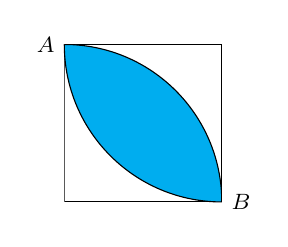
\begin{tikzpicture}[scale=2]
		\begin{scope}
			\clip (-1,0) rectangle (0,-1);
			\draw (-1,0) rectangle (0,-1);
			\clip (0,0) circle (1);			
			\draw[fill=cyan] (-1,-1) circle (1);			
		\end{scope}
		\path
		(-1,0) node[left]{\footnotesize$ A $}
		(0,-1) node[right]{\footnotesize $ B $}
		;
		\draw (0,-1) arc (-90:-180:1);
	\end{tikzpicture}\end{center}
Xét $\dfrac{1}{16}$ viên gạch men (vùng hình vuông chứa một cánh hoa).\\
Vì phần cánh hoa (màu xanh) là phần giao nhau của các đường tròn có khoảng cách giữa các tâm là $20\sqrt{2}$ nên một cánh hoa là phần giao của hai phần tư hình tròn tâm $A$, $B$ (hình vẽ), có bán kính $r=20$.\\
Mỗi phần tư hình tròn tâm $A$, $B$ có diện tích $S=\dfrac{1}{4}\pi \cdot 20^2$.\\
Diện tích hình vuông có $AB$ là đường chéo $S_\text{hình vuông}=20^2$.\\
Suy ra diện tích của một cánh hoa là $2S-S_\text{hình vuông}=\dfrac{1}{2}\pi \cdot 20^2-20^2=\left( \dfrac{\pi }{2}-1 \right)\cdot 20^2$.\\
Do đó
\begin{itemize}
	\item Diện tích phần màu xanh là $S_1=16\cdot\left( \dfrac{\pi}{2}-1\right)\cdot20^2$.
	\item Diện tích phần màu trắng $S_2=80^2-S_1$ cm$^2$.
\end{itemize}	
Số tiền tráng men một viên gạch là $T=5S_1+3S_2=26\,506{,}192\,98$ đồng.\\
Để sản xuất $100\,000$ viên gạch thì số tiền tráng men là $100\,000T=2\,650\,619\,298$ (nghìn đồng) xấp xỉ $2{,}65$ tỉ đồng.}
	\end{ex}
\Closesolutionfile{ans}

\indapan{6}{ans/ans-25-2-ThaiBinh-SoGD-L1-LC}
\indapan{4}{ans/ans-25-2-ThaiBinh-SoGD-L1-DS}
\indapan{6}{ans/ans-25-2-ThaiBinh-SoGD-L1-KQ}
